\chapter{Link--Discovery--Framework}
\label{ld_framework}

\emph{Link Discovery} \cite{na2011, vbgk2009}, oder \emph{Link Prediction} \cite{twak2003, nk2007}, bezeichnet Methoden des Data Minings \cite{hkp2012}, die zum Ziel haben, Verbindungen zwischen Objekten herzustellen. Diese Verbindungen werden aus vorhandenen Daten abgeleitet.

Das folgende Kapitel beschreibt das Framework, das für die Link Discovery im Rahmen dieser Arbeit angewendet wurde. Das Framework beschreibt die Kombination aus dem modellierten Weltausschnitt, dem Prozess zur Herstellung der Beziehungen, Kookkurrenz als Maß für Beziehungen, Graphen als Mittel zur Beschreibung des Weltausschnittes, möglichen Datenquellen und evolutionären Algorithmen als Mittel zur Priorisierung der erzeugten Beziehungen.

\section{Modell des Weltausschnittes}
\label{world_model}

Der folgende Abschnitt beschäftigt sich mit der Modellierung des im Rahmen dieser Arbeit verwendeten Weltausschnittes. Das Entity--Relationship--Diagramm des resultierenden Modells ist in \cref{fig:world_model} dargestellt.

\begin{figure}
\centering
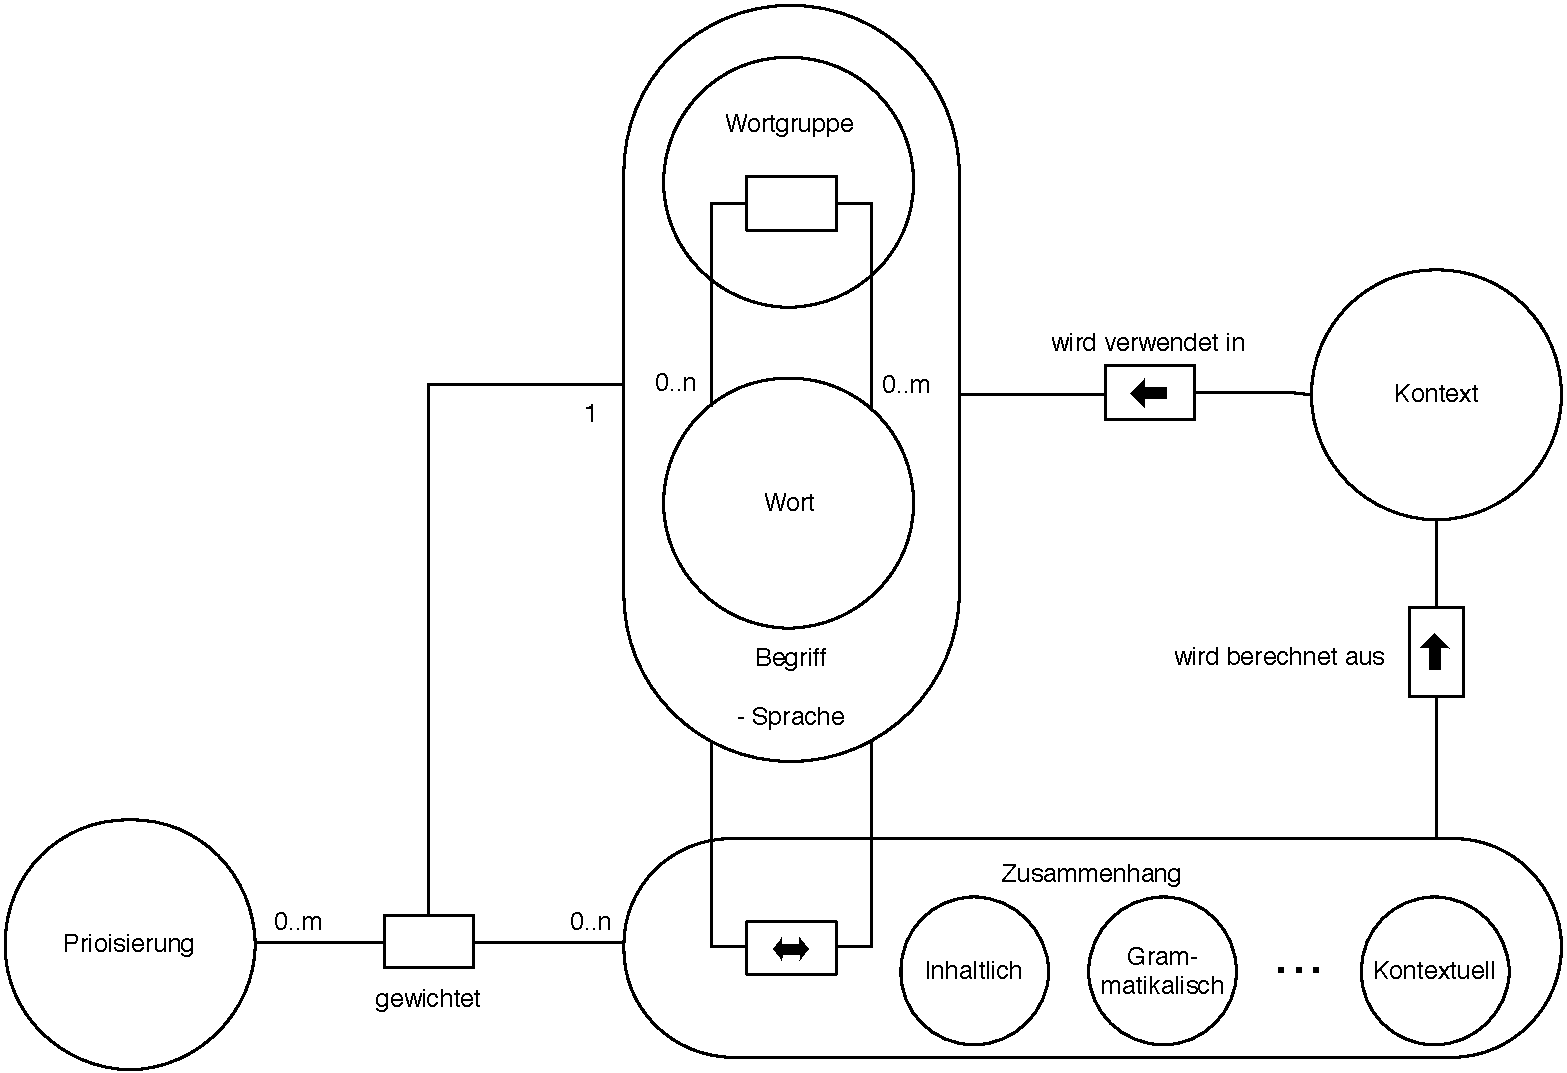
\includegraphics[width=\textwidth]{abstract_world_model}
\caption{FMC--Entity--Relationship--Diagramm des Modells des Weltausschnittes}
\label{fig:world_model}
\end{figure}

Zentrale Entität des Modells ist der \emph{Begriff}. Ein Begriff repräsentiert ein Einzelwort oder eine Wortgruppe in einer bestimmten Sprache. Dies berücksichtigt den Umstand, dass Wörter in mehreren Sprachen vorkommen können, jedoch in den jeweiligen Kulturräumen verschiedene Bedeutungen besitzen. Wortgruppen können aus beliebig vielen Einzelwörtern zusammengesetzt sein. Mit Hilfe der Link Discovery sollen zwischen diesen Begriffen verschiedenartige \emph{Zusammenhänge} gefunden werden.

Ein Zusammenhang (oder \emph{Beziehung}) besteht immer zwischen genau zwei Begriffen und besitzt einen bestimmten \emph{Typ}. Der Typ bezeichnet die Art des Zusammenhangs zwischen diesen beiden Begriffen. Beispiele für Zusammenhangstypen sind inhaltliche Zusammenhänge wie Synonyme, grammatikalische Zusammenhänge wie Wort-- und Grundformen oder kontextuelle Zusammenhänge, die sich aus der Verwendung des Begriffes ergeben. Dabei kann ein Zusammenhang, abhängig vom Typ, Attribute besitzen, die den Zusammenhang genauer spezifizieren. Dies kann beispielsweise ein Gewicht des Zusammenhangs sein, das die Wichtigkeit gegenüber anderen Beziehungen gleichen Typs angibt.

Je nach Nutzungsform der Daten wird unter Umständen eine andere Sicht auf die Beziehungen benötigt. Eine \emph{Priorisierung} stellt eine Gewichtung der Beziehungen eines Begriffes nach Typ dar. Sie teilt jeder Zusammenhangsart ein Gewicht relativ zu den anderen Arten zu. Somit werden durch die Priorisierung bestimmte Zusammenhänge höher gewichtet als andere. Die Priorisierung wird zu einer auf den Anwendungsfall abgestimmten Ordnung der Beziehungen eines Begriffes genutzt.

Die Verwendung eines Begriffes wird durch den \emph{Kontext} beschrieben. Dieser Kontext repräsentiert, wie der Begriff innerhalb einer bestimmten Anwendungsdomäne verwendet wurde. Daher sind die Attribute, die ein Kontext besitzen kann, nicht vorab spezifizierbar. Sie hängen von der jeweiligen Anwendungsdomäne ab. Beispiele für Kontexte sind die Verwendung eines Begriffes in einem Tagging--System oder in einer Ontologie. Aus diesem Kontext werden im Laufe der Link Discovery Zusammenhänge berechnet.

Dieses Modell bildet die Grundlage für den im folgenden Abschnitt beschriebenen Link--Discovery--Prozess.

\section{Link--Discovery--Prozess}
\label{ld_process}

Der Link--Discovery--Prozess beschreibt die Abfolge von Schritten, die zur Erzeugung und Anreicherung des in \cref{world_model} beschriebenen Weltausschnittes durchgeführt werden. Er dient somit zur Erzeugung von Begriffen und deren Zusammenhängen. \cref{fig:link_discovery_process} zeigt den Prozess als Petri--Netz.

\begin{figure}
\centering
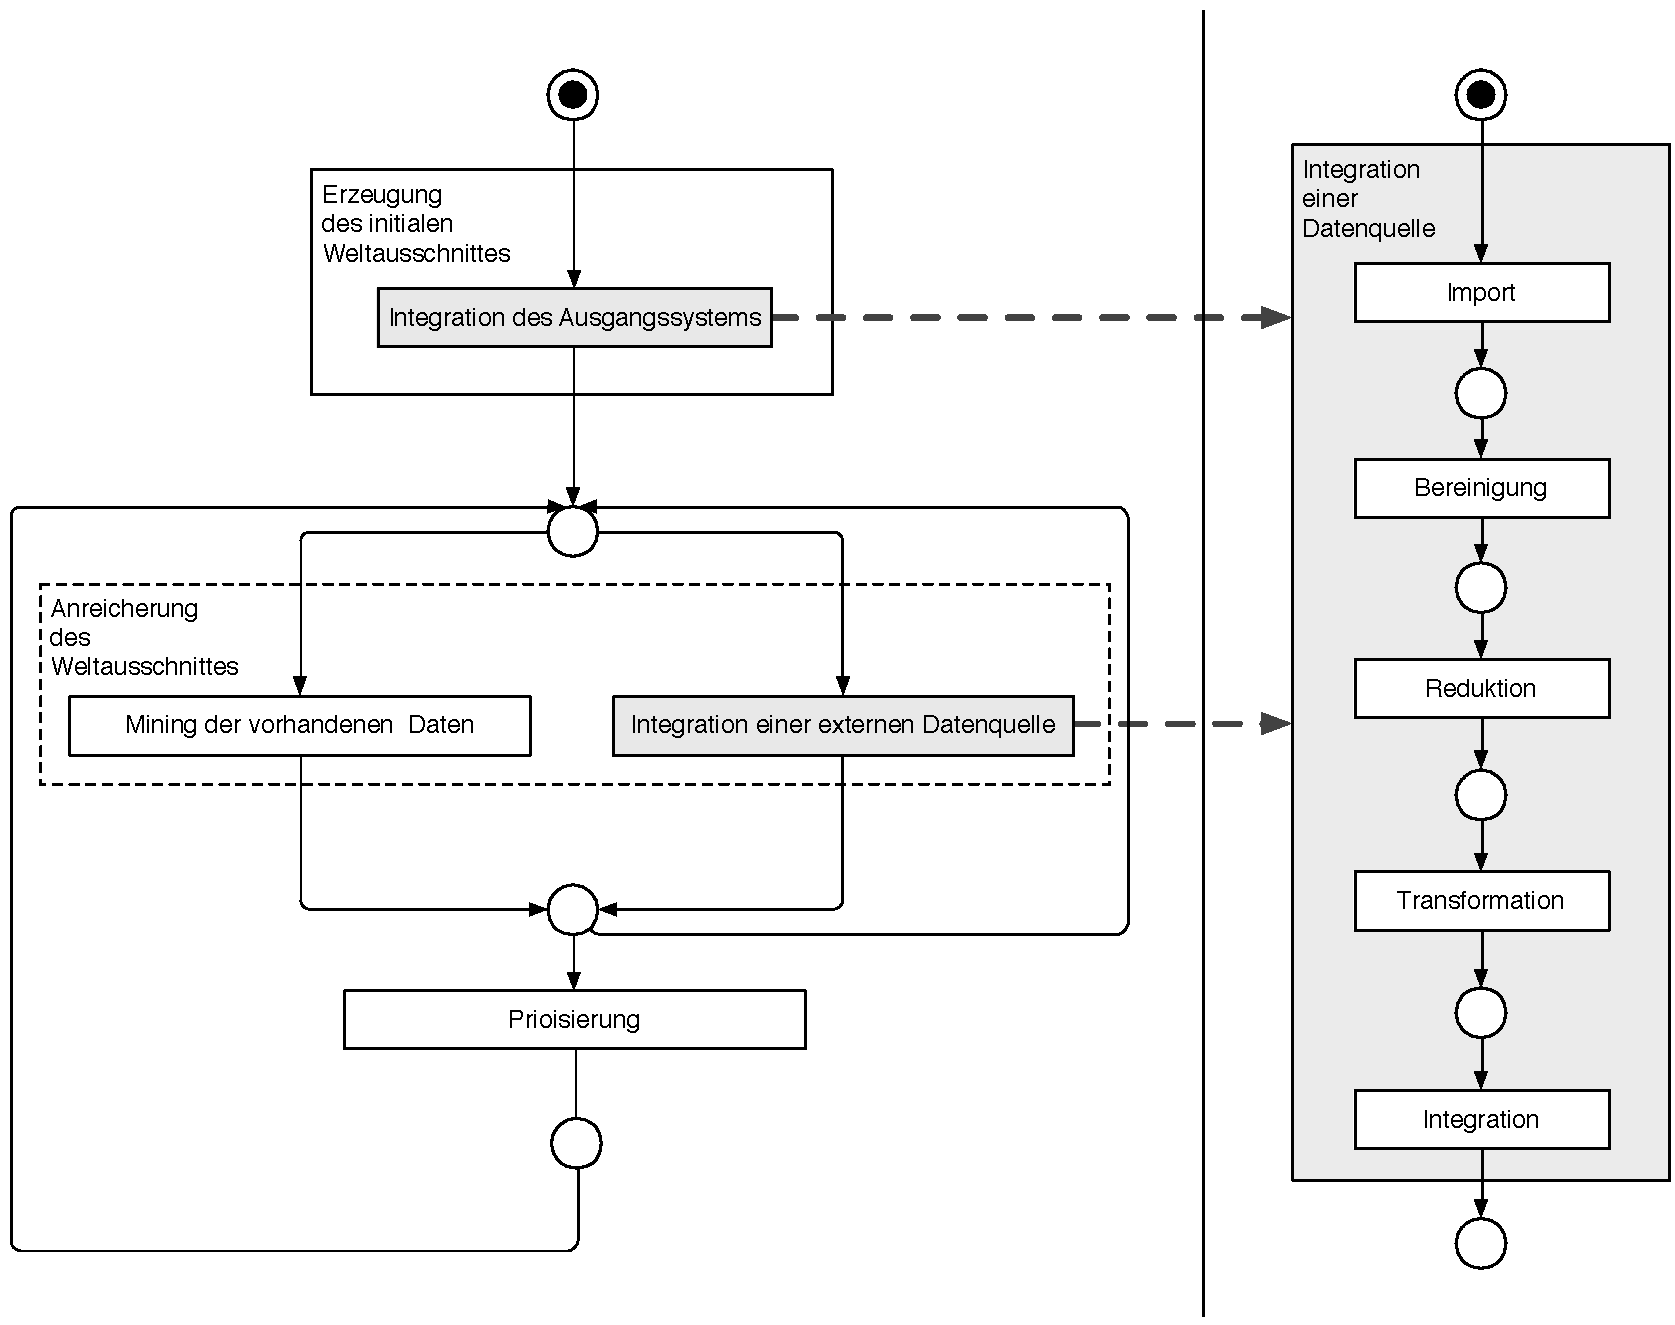
\includegraphics[width=\textwidth]{link_discovery_process}
\caption{FMC--Petri--Netz des Link--Discovery--Prozesses}
\label{fig:link_discovery_process}
\end{figure}

Die grundlegenden Phasen des Prozesses sind die initiale \emph{Erzeugung} des Weltausschnittes, dessen \emph{Anreicherung} und die \emph{Priorisierung} der Beziehungen. Sowohl bei der initialen Erzeugung als auch bei der Anreicherung wird ein Prozess zur Integration von Datenquellen benötigt.

Die Schritte der Anreicherung und Priorisierung können beliebig oft wiederholt werden, um das Ergebnis zu verbessern und auf die gewünschte Anwendung anzupassen. Die Anreicherung kann grundsätzlich durch das Mining der bereits im Weltausschnitt vorhandenen Daten oder durch die Integration neuer Datenquellen erfolgen.

Die genannten Schritte werden in den folgenden Abschnitten erläutert.

\subsection{Integration von Datenquellen}
\label{integration_generic}

Für die Link Discovery wird ein einheitliches Vorgehen zur Integration von Datenquellen benötigt. Die Datenquellen stellen grundsätzlich für die Link Discovery nützliche Daten zur Verfügung, die jedoch im Allgemeinen noch nicht direkt dem Modell des Weltausschnittes entsprechen. Demzufolge müssen diese Daten entsprechend verarbeitet werden.

Die zur Integration von externen Datenquellen nötigen Schritte entsprechen im Wesentlichen den von \textcite[S. 48f.]{hkp2012} beschriebenen Aufgaben der Datenvorverarbeitung: \emph{Bereinigung}, \emph{Reduktion}, \emph{Transformation} und \emph{Integration}. Diesen wird in dieser Arbeit der Schritt \emph{Import} vorangestellt, da es nicht immer möglich oder nötig ist, den gesamten Datenbestand einer Datenquelle zu nutzen. Somit sollten im Importschritt auch die Anfragen an die Datenquelle spezifiziert werden. Die genannten Schritte werden zur Link Discovery immer in der genannten Reihenfolge ausgeführt und werden im folgenden kurz beschrieben.

\paragraph{Import}

Im Importschritt werden die Rohdaten aus der Datenquelle extrahiert. Dabei wird die Form der Daten nicht verändert. Ist es nicht möglich oder nötig, den gesamten Datenbestand einer Quelle zu importieren, so muss eine Auswahl der anzufragenden Daten formuliert werden. Diese Auswahl richtet sich nach Möglichkeit nach den bereits im Weltausschnitt vorhandenen Daten. Beispielsweise können die Anfragen an die Datenquelle den bereits im Weltausschnitt gespeicherten Begriffen entsprechen.

\paragraph{Bereinigung}

Im nachfolgenden Bereinigungsschritt werden die importierten Daten so gut wie möglich von eventuell vorhandenen Defekten bezüglich der Datenqualität (siehe auch \cref{quality}) befreit. Dazu zählen beispielsweise die Entfernung von nicht nutzbaren Zeichen oder unvollständigen Datensätzen.

\paragraph{Reduktion}

Der Reduktionsschritt dient zur Verkleinerung der Datenmenge. Dazu gehören beispielsweise Schritte zur Duplikatentfernung oder zur Auswahl relevanter Datensätze. In dieser Arbeit bestand die Haupteinschränkung der Datenmenge darin, nach Möglichkeit nur deutschsprachige Begriffe auszuwählen.

\paragraph{Transformation}
\label{transformation}

Der Schritt der Transformation überführt die Daten schließlich in das Modell des Weltausschnittes. Dies bedeutet, dass die Datensätze in Begriffe und Beziehungen umgewandelt werden. Dabei sollten möglichst viele Informationen über den Kontext der Begriffe erhalten bleiben. Die Methode, nachder diese Transformation vorgenommen wird, hängt von der Datenquelle ab. Generell werden die Beziehungen meist aus dem Kontext der Begriffe, wie er in der Datenquelle vorliegt, gebildet. Ein Mittel für die Beziehungserzeugung ist die Kookkurrenz, welche in \cref{co-occurence} erläutert wird. Somit stellt der Transformationsschritt die wichtigste Komponente für die Integration einer Datenquelle dar.

\paragraph{Integration}

Der Integrationsschritt für jede Datenquelle dient letztendlich der Zusammenführung des im Transformationsschritt erzeugten Weltausschnittes mit dem bereits vorhandenen Weltausschnitt. Dabei werden bereits existierende Begriffe vereinigt und die neu erzeugten Beziehungen übernommen. Die Zusammenführung der Begriffe erfolgt über die Verknüpfung des existierenden Begriffes mit dem neu erzeugten Kontext, den die Datenquelle zu einem Begriff liefert.

\subsection{Initiale Erzeugung des Weltausschnittes}

Der erste Schritt der Link Discovery besteht in der Auswahl einer geeigneten Datenquelle für die initiale Erzeugung des Weltausschnittes. In dieser Arbeit ist diese Datenquelle das Tagging--System von Spreadshirt (siehe \cref{tag_sprd}).

Die Auswahl der Datenquelle richtet sich im wesentlichen danach, ob der Kontext, den die Datenquelle potenziell zu Begriffen liefern kann, für die Link Discovery geeignet ist. Der Kontext sollte außerdem für die geplante Anwendung der Ergebnisse der Link Discovery relevant sein.

Nach der Auswahl einer geeigneten Quelle werden die in \cref{integration_generic} beschriebenen Schritte zur Integration durchgeführt. Der Schritt der Integration ist trivial, da zu diesem Zeitpunkt noch keine Daten im Weltausschnitt vorhanden sind.

\subsection{Anreicherung des Weltausschnittes}

Nach der initialen Erzeugung des Weltausschnittes kann dieser mit beliebig vielen Anreicherungsschritten ergänzt werden. Unter Anreicherung wird die Erzeugung neuer Begriffe, Kontexte oder Zusammenhänge verstanden.

Das Hinzufügen neuer Begriffe erweitert das Vokabular des Weltausschnittes. Somit können bei der Benutzung der Daten zu einer größeren Menge von Begriffen Zusammenhänge gefunden werden. Die Erzeugung von Kontexten zu vorhandenen oder neuen Begriffen erweitert das Wissen über die Benutzung eines Begriffes innerhalb einer bestimmten Anwendungsdomäne. Die Anreicherung des Weltausschnittes mit neuen Zusammenhängen ermöglicht einerseits das Finden von relevanten Nachbarn eines Begriffes, erfordert andererseits jedoch, abhängig von der Anwendung, auch eine andere Priorisierung der Zusammenhangstypen.

Grundsätzlich kann die Anreicherung des Weltausschnittes auf zwei Arten erfolgen. Dies ist zum Einen die Anreicherung durch das Mining der bereits vorhandenen Daten, zum Anderen die Anreicherung durch Integration einer weiteren Datenquelle.

\subsubsection{Anreicherung durch Mining vorhandener Daten}
\label{enrichment_mining}

Die Erzeugung neuer Begriffe und Zusammenhänge kann aus den vorhandenen Daten mittels Methoden des Data Minings vorgenommen werden. Dazu werden die bereits im Weltausschnitt vorhandenen Begriffe mit ihren Kontexten und Beziehungen analysiert, um bisher unbekannte Zusammenhänge zu finden.

Beispiele für anwendbare Methoden sind hierbei Assoziationsanalyse \cite[S. 328f.]{pt2013} oder Clusteranalyse \cite[S. 443f.]{hkp2012}, um bestimmte, bereits in den Daten vorhandene, aber nicht explizit abgebildete Zusammenhänge zu ermitteln. Jedoch können auch einfachere Methoden wie die Zerlegung von Wortgruppen in Einzelwörter (siehe \cref{decomposition}) oder das Einfügen von bisher nur transitiv, also nur über mehrere Begriffe, vorhandenen Beziehungen erfolgreich sein, um neue Begriffe und Beziehungen in den Datenbestand einzuführen.

\subsubsection{Anreicherung durch Integration externer Datenquellen}
\label{enrichment_external}

Sofern weitere Datenquellen verfügbar sind, stellt deren Integration einen weiteren erfolgversprechenden Weg dar, um die Daten anzureichern. Neue Datenquellen beschreiben immer einen neuen Kontext, in dem Begriffe genutzt werden. Ist der Kontext dieser Begriffe für die spätere Anwendung relevant, ist die Integration der jeweiligen Datenquelle zu Zwecken der Link Discovery von großem Interesse.

Um die zusätzliche Datenquelle zur Link Discovery zu nutzen, werden die Schritte, die schon zur initialen Erzeugung des Weltausschnittes zum Einsatz kamen, genutzt (siehe \cref{integration_generic}). Dazu werden im Transformationsschritt Daten erzeugt, die dem Modell des Weltausschnittes entsprechen. Im Integrationsschritt werden sie mit den bereits vorhandenen Daten zusammengeführt.

\subsection{Priorisierung von Beziehungen}
\label{prioritization}

Ziel des Priorisierungsschrittes der Link Discovery ist das Finden einer Gewichtung der Zusammenhangstypen, die für einen Anwendungsfall relevante Nachbarn zu einem Begriff liefert. Die Relevanz kann jedoch nur von einem Benutzer bewertet werden. \cref{fig:prioritization} stellt den Priorisierungsprozess dar.

\begin{figure}
\centering
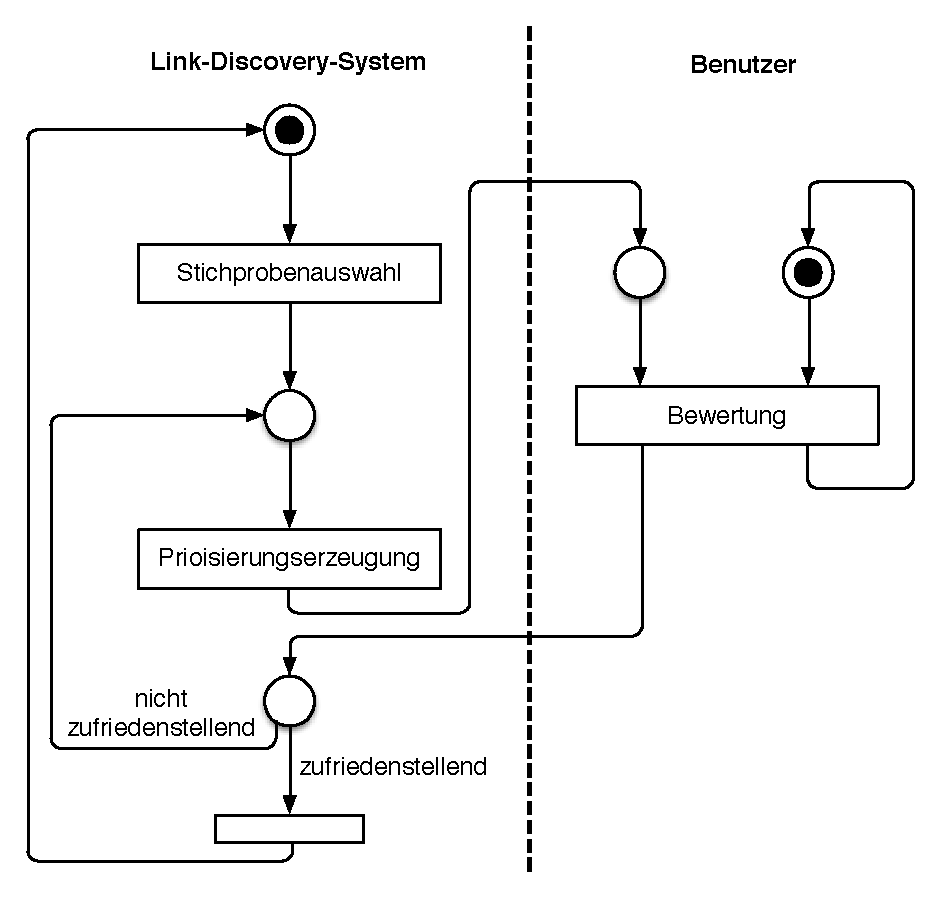
\includegraphics[width=0.7\textwidth]{prioritization}
\caption{FMC--Petri--Netz der Priorisierung}
\label{fig:prioritization}
\end{figure}

Grundsätzlich kann nicht davon ausgegangen werden, dass eine Priorisierung für alle im Weltausschnitt gespeicherten Begriffe relevante Nachbarn liefert. Daher sollte die Priorisierung stichprobenhaft für einzelne Begriffe durchgeführt werden, um dann möglicherweise eine global gute Ergebnisse liefernde Priorisierung zu ermitteln.

Der Priorisierungsprozess beginnt mit der Auswahl einer Stichprobe anhand geeigneter Kriterien für das Anwendungsszenario. Beispielhaft für Kriterien sind externe Faktoren wie die Popularität des Begriffes in der Anwendungsdomäne oder im Weltausschnitt gespeicherte Faktoren wie die Anzahl der Zusammenhänge, die ein Begriff besitzt. Wird der Prozess mit mehreren Stichproben durchgeführt, sollte auf eine möglichst breite Streuung des jeweiligen Kriteriums geachtet werden, um die Güte der Priorisierungen abhängig vom Begriff beurteilen zu können.

Nach der Auswahl der Stichprobe wird vom Link--Discovery--System eine Priorisierung erzeugt. Wie diese Erzeugung konkret implementiert ist, hängt von der Anwendung ab. Im Rahmen dieser Arbeit wurden evolutionäre Algorithmen (siehe \cref{evo_for_prio}) gewählt. Die erzeugte Priorisierung wird auf den Begriff angewendet und von einem Benutzer bewertet. Der Benutzer sollte Wissen über die Anwendungsdomäne besitzen.

Ist die Bewertung der Priorisierung positiv, ist der Priorisierungsprozess beendet. Bei nicht zufriedenstellendem Ergebnis wird die Erzeugung einer neuen Priorisierung und die anschließende Bewertung wiederholt. Stellt sich auch nach einer im Voraus gewählten Anzahl von Iterationen dieser Art kein zufriedenstellendes Ergebnis ein, so sollte die Priorisierung abgebrochen und die Gründe für das Fehlschlagen analysiert werden. Diese können beispielsweise in einer schlechten Qualität der Beziehungen des Weltausschnittes, in einer unpassenden Stichprobenauswahl oder fehlendem Wissen des Benutzers gefunden werden.

\section{Kookkurrenz als Mittel zur Beziehungserzeugung}
\label{co-occurence}

Im Transformationsschritt der Link Discovery (\cref{transformation}) wird eine Methode benötigt, um aus dem Kontext von Begriffen Beziehungen zwischen eben jenen zu berechnen. Eine der möglichen Methoden ist die Berechnung von \emph{Kookkurrenz}. Diese wird im folgenden Abschnitt näher erläutert.

\subsection{Grundlagen von Kookkurrenz}

Um gewichtete inhaltliche Beziehungen zwischen Begriffen herstellen zu können, wird eine Definition von \emph{Ähnlichkeit} benötigt. Diese lässt sich auf vielfältige Arten bestimmen.

\begin{figure}
\centering
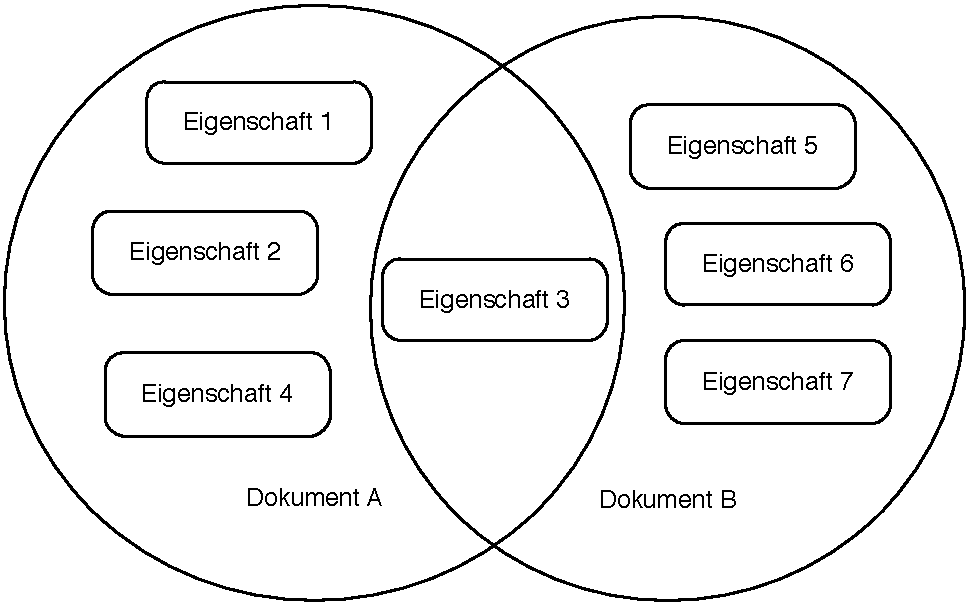
\includegraphics[width=0.5\textwidth]{similarity}
\caption{Repräsentation von Dokumenten als Mengen von Eigenschaften}
\label{fig:similarity}
\end{figure}

Die Ähnlichkeit zwischen zwei Dokumenten kann grundsätzlich nach \textcite{at1977} definiert werden. Dieser Definition liegt zu Grunde, dass sich die Dokumente als Mengen von Eigenschaften beschreiben lassen. Im Gegensatz zu anderen Ähnlichkeitsmodellen hängt die Ähnlichkeit nicht nur von den gemeinsamen Eigenschaften der Dokumente ab, sondern auch von den Eigenschaften, die die Dokumente allein besitzen. Diese Definition von Ähnlichkeit wird in \cref{fig:similarity} veranschaulicht.

\label{similarity}
Somit lässt sich Ähnlichkeit \(s(A,B)\) zwischen den Dokumenten, die durch die Mengen \(A\) und \(B\) dargestellt werden, definieren durch:
\[s(A,B) = F(A \cap B, A-B, B-A)\]

Die Gestaltung der Funktion \(s\) und die Auswahl der für die Ähnlichkeitsberechnung genutzten Eigenschaften der Dokumente hängt stark von der Anwendung ab. Somit beschreibt beispielsweise die Levenshtein--Distanz \cite{vl1966} die Ähnlichkeit zweier Zeichenketten durch die minimale Menge von Einfüge-, Lösch- und Ersetzungsoperationen, die nötig sind, um eine Zeichenkette in die andere umzuwandeln. In Ontologien und Taxonomien kann die Ähnlichkeit von Begriffen mittels der Knoten- oder Kanteneigenschaften berechnet werden. Beispiele hierfür sind die Ähnlichkeit in Ontologien nach \textcite{pr1995} und \textcite{ps2002}. In der Bildverarbeitung können merkmalsbasierte Ähnlichkeitsmaße ebenfalls eingesetzt werden, beispielsweise beschreiben \textcite{ow2006} ein Ähnlichkeitsmaß auf Basis von Clusteringalgorithmen, die auf Rastergrafiken angewandt werden.

Im Rahmen dieser Arbeit wird ein Ähnlichkeitsmaß gesucht, das anhand der Eigenschaften von Begriffen eine Distanz zwischen diesen berechnet. Da eine inhaltliche Ähnlichkeit gesucht wird, spielen linguistische Ähnlichkeitsmaße wie die Levenshtein--Distanz eine untergeordnete Rolle. Zu Beginn bestehen keinerlei Verbindungen zwischen den Begriffen, so dass keine Ähnlichkeitsmaße für Ontologien eingesetzt werden können. Somit bietet sich die Wahl eines Ähnlichkeitsmaßes an, das den Kontext, in dem die Begriffe im Quellsystem verwendet werden, berücksichtigt.

In \cref{tag_sprd} wurde das für diese Arbeit verfügbare Tagging--System beschrieben. In diesem System besitzen die Tags wenig Kontext. Die einzig verfügbare Information ist, an welche Dokumente die Tags vergeben wurden.

Wenn mehrere Begriffe pro Dokument verwendet werden, wird damit ein Zusammenhang zwischen den Begriffen beschrieben. Dieser Zusammenhang lässt sich mit dem Ähnlichkeitsmaß \emph{Kookkurrenz} messen. Kookkurrenzmaße beschreiben, wie oft Begriffe gemeinsam verwendet werden \cite[S. 21]{zz2011}. Dies wird ins Verhältnis zum einzelnen Auftreten der Begriffe gesetzt und genügt somit der Definition von Ähnlichkeit in \cref{similarity}.

Hierzu muss angemerkt werden, dass die Ähnlichkeit mittels Kookkurrenz nicht zwingend eine Ähnlichkeit der den Begriffen zu Grunde liegenden Konzepte darstellt. Die Verwendung von Kookkurrenz als Ähnlichkeitsmaß beruht allein auf der Annahme, dass Menschen zur Beschreibung von gleichen Inhalten die gleichen Begriffe benutzen. Diese Annahme muss im Laufe der Evaluierung der Ergebnisse validiert werden.

\subsection{Maße für Kookkurrenz}
\label{measures}

Werden die Objekte, zwischen denen die Ähnlichkeit berechnet werden soll, als Mengen von Eigenschaften definiert, bieten sich die üblichen Kennzahlen für die Ähnlichkeiten von Mengen an. Ein Begriff kann als Menge der Dokumente, für die er als Beschreibung verwendet wurde, definiert werden.

Um die Ähnlichkeit zwischen zwei Begriffen zu ermitteln, lassen sich die Vereinigungsmenge, Schnittmenge und Kreuzprodukte der jeweiligen Mengen bilden, die die Begriffe repräsentieren. Ist \(A\) die Menge der Dokumente, die mit einem Begriff \(a\) versehen wurden, \(B\) die Menge der Dokumente mit einem Begriff \(b\), so ergeben sich die Mengen:

\begin{itemize}
    \item \(A \cap B\), alle Dokumente die mit \(a\) und \(b\) versehen wurden
    \item \(A \cup B\), alle Dokumente die mit \(a\) oder \(b\) versehen wurden
    \item \(A \times B\), alle Dokumentenpaare, die sich aus den Mengen \(A\) und \(B\) bilden lassen
\end{itemize}

Die Mächtigkeiten dieser Mengen können dann zur Berechnung verschiedener Ähnlichkeitsmaße verwendet werden. Drei der üblichsten Maße wurden im Rahmen dieser Arbeit verwendet und werden im Folgenden genannt.

\subsubsection{Sørensen--Dice}

Der Sørensen--Dice--Koeffizient \cite{st1948} \cite{ld1945}, oft auch nur als Dice--Koeffizient bezeichent, entstand ursprünglich in der Biologie und wurde verwendet, um die Ähnlichkeit zwischen Proben zu berechnen. Heute findet er allgemeine Anwendung im Data Mining. Er ist definiert durch:

\[
\delta_{Dice}(a, b) = \frac{2|A \cap B|}{|A|+|B|}
\]

Der Wertebereich \(W\) des Koeffizienten wird mit \(W=[0,1] \in \mathbb{R}\) angegeben.

\subsubsection{Jaccard}

Der Jaccard--Index \cite{pj19012} wurde ursprünglich mit dem gleichen Zweck wie der Dice--Koeffizient verwendet. Sein Wertebereich wird ebenfalls mit \(W=[0,1] \in \mathbb{R}\) angegeben und er ist definiert durch:

\[
\delta_{Jaccard}(a,b) = \frac{|A \cap B|}{|A \cup B|}
\]

\subsubsection{Kosinus}

Die Kosinus-Ähnlichkeit \cite{hkp2012} ist ursprünglich ein Maß für die Ähnlichkeit zweier Vektoren. Sie ist eine Maßzahl dafür, ob die Vektoren ungefähr in die gleiche Richtung zeigen. Sie kann jedoch genauso auf Mengen angewendet werden, da das Vorhandensein der Elemente in der Menge auch durch einen Vektor in einem \(n\)-dimensionalen Raum dargestellt werden kann, wobei \(n\) die Anzahl aller möglichen Eigenschaften ist. Der Wertebereich der Kosinus-Ähnlichkeit ist ebenfalls mit \(W=[0,1] \in \mathbb{R}\) angegeben. Sie ist auf den in \cref{measures} definierten Mengen definiert durch:

\[
\delta_{Cosine}(a, b) = \frac{|A \cap B|}{\sqrt{|A| \times |B|}}
\]

Nachdem die Ähnlichkeit mittels Kookkurrenz und die entsprechenden Maße vorgestellt wurden, wird im nächsten Abschnitt die Berechnung und damit verbundene Komplexität diskutiert.

\subsection{Berechnung von Kookkurrenz}

Um die in \cref{measures} genannten Maße für Kookkurrenz zu berechnen, muss das Kreuzprodukt aller Begriffe gebildet werden. Dabei muss für jedes Paar von Begriffen die Häufigkeit gezählt werden, wie oft die Begriffe gemeinsam zur Beschreibung von Dokumenten verwendet wurden. Diese Häufigkeit beschreibt die Mächtigkeit der Mengen \(A \cap B\). Außerdem muss gezählt werden, wie oft jeder Begriff insgesamt verwendet wird, um die Mächtigkeit der Mengen \(A, B, \dots\) zu bestimmen. Danach können über die genannten Formeln die Kookkurrenzmaße berechnet werden. In \cref{lst:coocc-pseudo} ist die Berechnung als Pseudo--Code dargestellt.

\begin{lstlisting}[language=pseudo, label={lst:coocc-pseudo}, caption={Kookkurrenzberechnung}, float]
var occurences = {};

foreach (term in terms) {
    occurences[term] = countOccurrences(term);
}

foreach (termA in terms) {
    foreach (termB in terms) {
        var ab = countCoOccurences(termA, termB);
    }
    var diceAB = dice(occurences[termA], occurences[termB], ab);
    var jaccardAB = jaccard(occurences[termA], occurences[termB], ab);
    var cosineAB = cosine(occurences[termA], occurences[termB], ab);
}
\end{lstlisting}

Der Aufwand, um die Kookkurrenzmaße für alle Paare von Begriffen zu berechnen, hängt von der Anzahl der Begriffe, Dokumente und Verwendungen ab. Beträgt die Anzahl der Begriffe \(n\) und die Anzahl der Dokumente \(d\), so ergibt sich für den Fall, dass jeder Begriff an jedes Dokument vergeben wurde eine Laufzeit von \(O(d*n^2)\). Wurden keine Begriffe mit Dokumenten verknüpft, beträgt die Laufzeit \(\Theta(d)\). Die reale Laufzeit der Ähnlichkeitsberechnung liegt daher zwischen diesen Schranken.

Es ist absehbar, dass der Rechenaufwand mit wachsender Datenmenge stark ansteigt. Somit scheint es ratsam, nach Optimierungen zu suchen, um die Rechenzeit zu verringern. Da sich die Anzahl der Berechnungen nicht vermindern lässt, kann eine Verkürzung der Rechenzeit nur durch Parallelisierung erreicht werden. Eine mögliche Umsetzung der parallelen Berechnung der Kookkurrenz mittels des Programmiermodells  MapReduce wird in \cref{mapreduce_cooccurence} erläutert.

\section{Graphen als Beschreibungsmittel des Weltausschnittes}
\label{graphs}

Nachdem in \cref{world_model} der zur Link Discovery verwendete Weltausschnitt modelliert wurde, wird zur Umsetzung eine Datenstruktur benötigt, die diesen Ausschnitt konkret abbildet. Da im Wesentlichen Objekte, zwischen denen Verbindungen bestehen, abgebildet werden, bietet sich die Verwendung eines Graphen an. Die Grundlagen von Graphen sowie die konkrete Abbildung des Weltausschnittes auf eine Graph--Datenstruktur werden in den folgenden Abschnitten erläutert.

\subsection{Grundlagen}
\label{graph_basics}

Ein \emph{ungerichteter Graph} ist definiert durch ein Paar \(G = (V,E)\) von Mengen, für die gilt: \(E \subseteq\ [V]^2\). Dies bedeutet, dass alle Elemente aus \(E\) 2-elementige Teilmengen von \(V\) sind \cite[S. 2]{rd2012}. Die Menge \(V\) repräsentiert die \emph{Knoten} und die Menge \(E\) die \emph{Kanten} des Graphen. Eine Kante stellt eine Verbindung von zwei Knoten dar. Zwei Knoten werden als \emph{Nachbarn} bezeichnet, wenn zwischen ihnen eine Kante existiert. \cref{fig:basic_graph} zeigt ein Beispiel für einen ungerichteten Graphen.

\begin{figure}
\centering
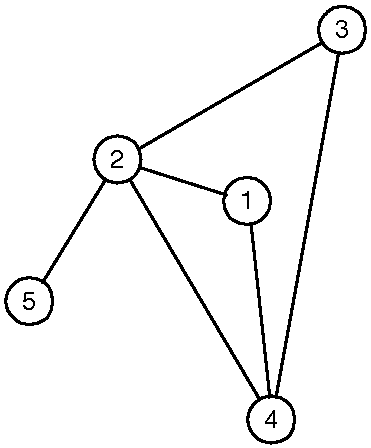
\includegraphics[width=0.2\textwidth]{basic_graph}
\caption{Ungerichteter Graph}
\label{fig:basic_graph}
\end{figure}

Ein \emph{gerichteter Graph} ist ein Graph, der neben den Mengen \(V\) und \(E\) die zwei Abbildungen \(quelle: E \rightarrow V\) und \(ziel: E \rightarrow V\) enthält \cite[S. 25]{rd2012}. Diese weisen jeder Kante \(e\) einen Quell- und Zielknoten zu. Die Kante ist somit von \(quelle(e)\) nach \(ziel(e)\) gerichtet. \cref{fig:directed_graph} zeigt einen gerichteten Graphen.

\begin{figure}
\centering
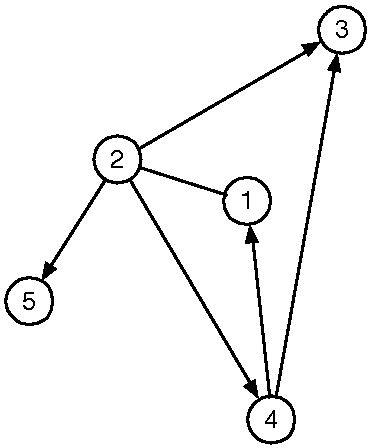
\includegraphics[width=0.2\textwidth]{directed_graph}
\caption{Gerichteter Graph}
\label{fig:directed_graph}
\end{figure}

Als \emph{Multigraph} wird schließlich ein Graph bezeichnet, bei dem zwischen zwei Knoten mehrere Kanten bestehen \cite[S. 25]{rd2012}. Sind diese gerichtet, spricht man vom einen \emph{gerichteten Multigraphen}. \cref{fig:directed_multigraph} illustriert einen solchen gerichteten Multigraphen.

\begin{figure}
\centering
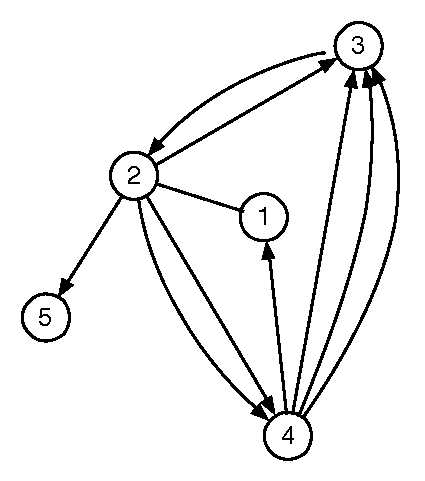
\includegraphics[width=0.2\textwidth]{directed_multigraph}
\caption{Gerichteter Multigraph}
\label{fig:directed_multigraph}
\end{figure}

Die Knoten und Kanten eines Graphen sind Objekte mit beliebigen weiteren Eigenschaften. Kanten besitzen üblicherweise ein Gewicht, das ihre Wichtigkeit oder Kosten im Anwendungskontext des Graphen angibt.

Nachdem Graphen grundsätzlich erläutert wurden, beschäftigt sich der folgende Abschnitt mit der konkreten Umsetzung des Modells des Weltausschnittes auf eine solche Graphen--Struktur.

\subsection{Graphenrepräsentation des Weltausschnittes}
\label{world_graph}

Um den Weltausschnitt in \cref{world_model} in eine Graphenform zur transformieren, muss zunächst modelliert werden, welche Objekte die Knoten und Kanten des Graphen repräsentieren.

\begin{figure}
\centering
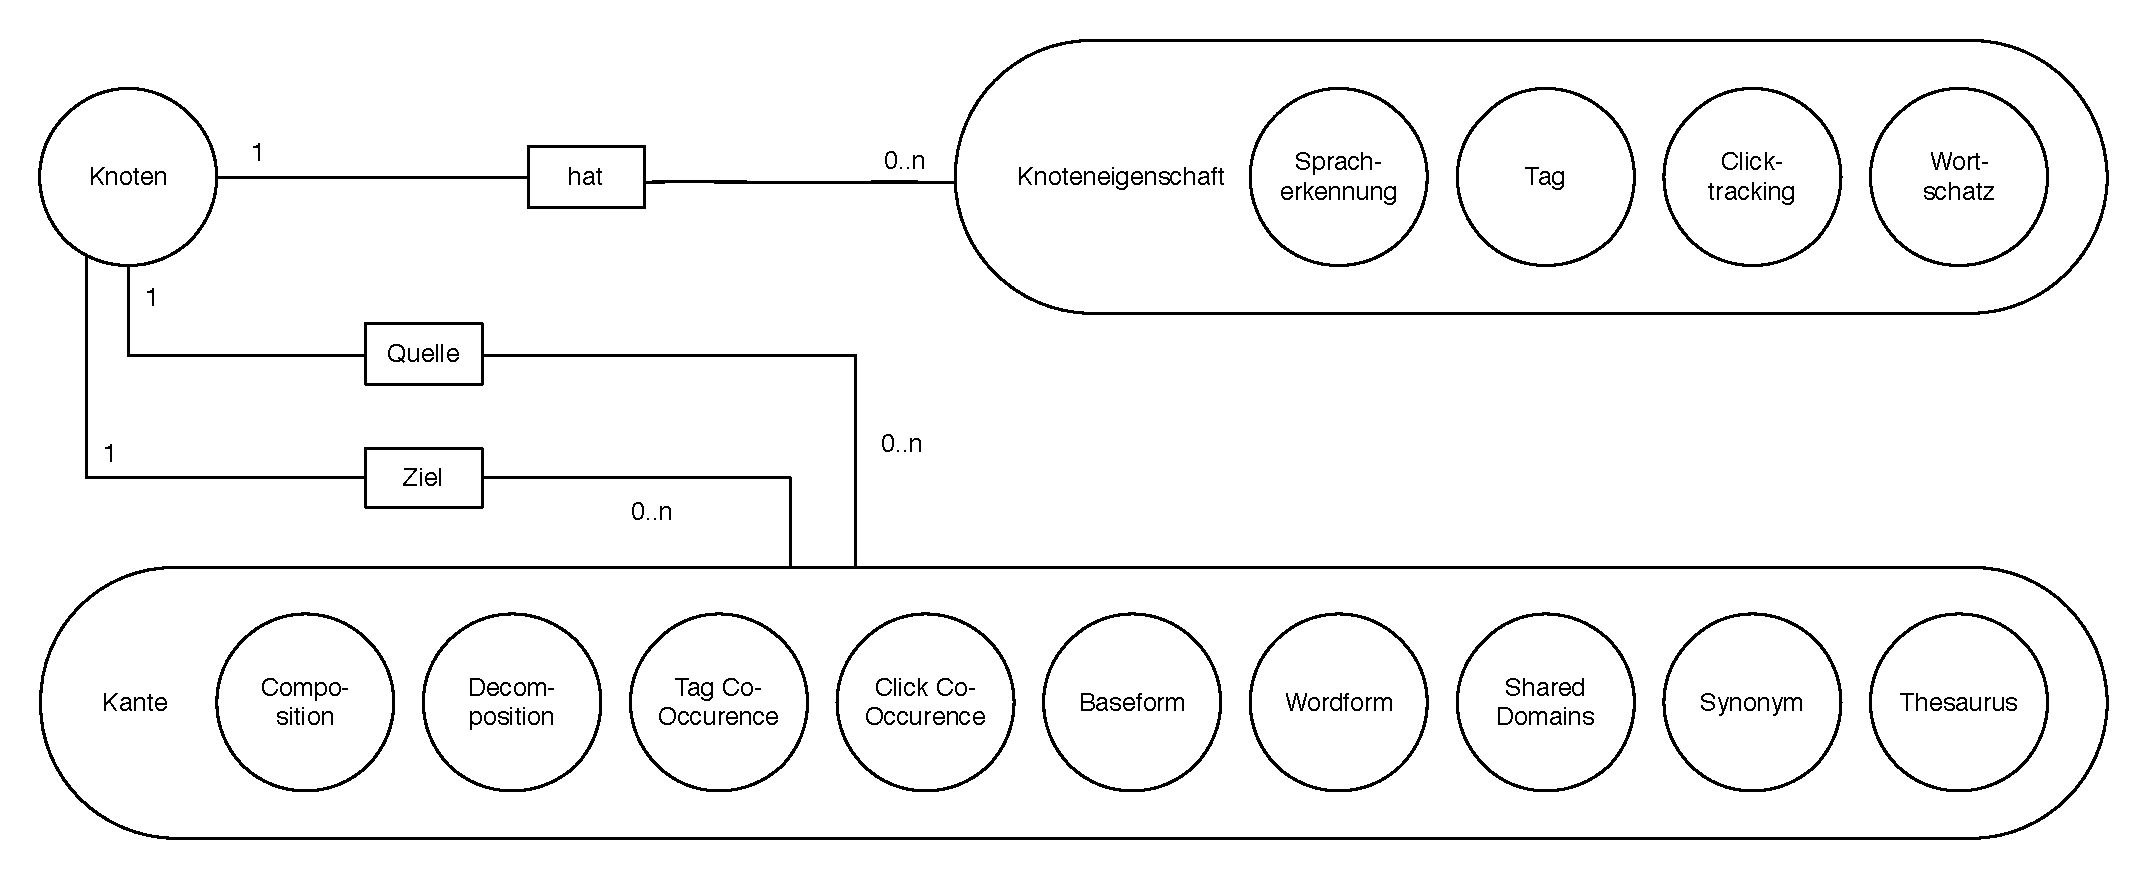
\includegraphics[width=1\textwidth]{graph_model}
\caption{FMC--Entity--Relationship--Diagramm der Graphenrepräsentation}
\label{fig:graph_model}
\end{figure}

Die Knoten repräsentieren die Begriffe, zwischen denen durch die Link Discovery Zusammenhänge hergestellt werden sollen. Sie enthalten als benötigte Attribute eine Zeichenkette und ein Attribut Sprache. Die Kombination dieser beiden Attribute ist innerhalb der Knotenmenge eindeutig, um je verwendetem Begriff in einer Sprache genau einen Knoten zu erhalten.

Der Kontext der Begriffe wird über Eigenschaften von Knoten abgebildet. Dabei kann ein Begriff beliebig viele Eigenschaften besitzen. Da die Kontexte der Begriffe aus jeweils einer Datenquelle stammen, bietet es sich an, pro Datenquelle eine Entität für die kontextuellen Eigenschaften, die diese Datenquelle liefert, zu definieren.

Eine Kante repräsentiert einen irgendwie gearteten Zusammenhang zwischen zwei Begriffen. Sie besitzt einen \emph{Typ}, der die Art des Zusammenhangs spezifiziert, sowie je einen Quell- und Zielknoten. Zusätzlich kann sie weitere Attribute besitzen. Bei Kanten, die durch Kookkurrenzberechnung (siehe \cref{co-occurence}) erzeugt wurden, sind dies beispielsweise die Anzahl des gemeinsamen Auftretens zweier Begriffe und die berechneten Kookkurrenzmaße. Im Rahmen dieser Arbeit wurden keine weiteren Attribute für Kanten benötigt, diese sind generell jedoch denkbar.

Zwischen zwei Knoten können beliebig viele, je Typ jedoch höchstens eine, Kanten existieren. Daher handelt es sich bei dem Graphen des Weltausschnittes um einen gerichteten Multigraphen (siehe \cref{graph_basics}).

Das resultierende komplette Modell des Graphen ist in \cref{fig:graph_model} dargestellt. Dieses beinhaltet sämtliche zum Zeitpunkt der Bearbeitung bekannten und integrierten Datenquellen und die damit verbundenen Kontexte und Kantentypen. Die Datenquelle des Tagging--Systems und der damit verbundene Kontext wird in \cref{tag_sprd} näher beschrieben. Das Clicktracking--System wird in \cref{clicktracking} und der Wortschatz der Universität Leipzig in \cref{wortschatz} näher beleuchtet. Details über die Erzeugung der entsprechenden Kantentypen werden in \cref{link_discovery} erläutert.

Um die Graphenrepräsentation des modellierten Weltausschnittes anschaulicher darzustellen, ist in \cref{fig:example_graph} ein beispielhafter Ausschnitt des nach Durchführung der Link Discovery entstehenden Graphen abgebildet. Auf Darstellung der Kontexte und Kantenattribute wurde aus Platzgründen verzichtet.

\begin{figure}
\centering
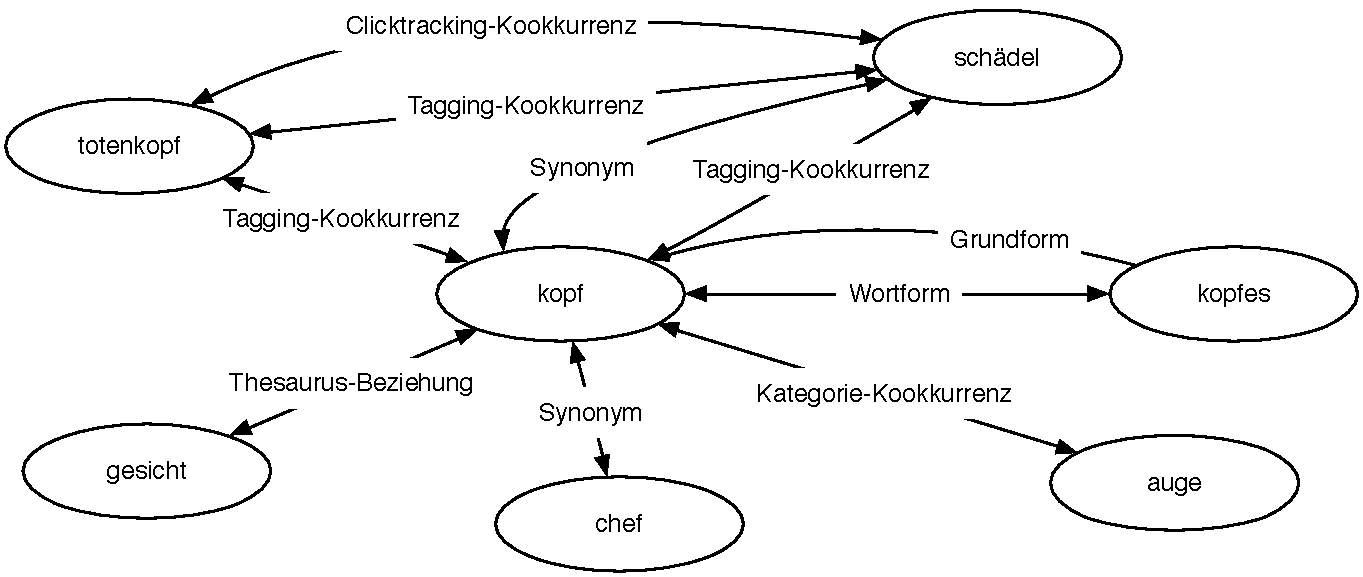
\includegraphics[width=\textwidth]{example_graph}
\caption{Beispiel--Graphausschnitt für das Ergebnis der Link Discovery}
\label{fig:example_graph}
\end{figure}

Nach der Definition der verwendeten Graphenstruktur werden im folgenden Abschnitt die möglichen Datenquellen diskutiert.

\section{Datenquellen zur Anreicherung}
\label{data_sources}

Der initiale Weltausschnitt wird im Rahmen dieser Arbeit aus den Daten des Tagging--Systems von Spreadshirt erzeugt. Wie in \cref{enrichment_external} bereits einführend erläutert, kann danach zur Anreicherung die Integration weiterer Datenquellen erfolgen. Diese Datenquellen können eine andere Sicht auf die Begriffe des Weltausschnittes liefern und somit zur Erzeugung neuer Beziehungen nützlich sein. In diesem Abschnitt werden mögliche Datenquellen genannt und erläutert sowie die letztendlich verwendeten Datenquellen näher beschrieben.

\subsection{Lexikalische Quellen}
\label{lexical_sources}

Da die Hauptentität des Weltausschnittes Begriffe einer Sprache darstellt, liegt es nahe, auf lexikalische Quellen zurückzugreifen. Diese existieren in unterschiedlichen Ausprägungen, haben jedoch alle gemeinsam, dass sie Wörter beschreiben und in Beziehung zu anderen Wörtern stehen. Damit eignen sie sich gut zur Integration in den Weltausschnitt. Einige der üblichen Formen von lexikalischen Quellen werden im folgenden genannt und erläutert.

Ein \emph{Wörterbuch} ist ein Nachschlagewerk, das erklärende Informationen über Wörter enthält \cite{hk2003}. Dabei kann es sich um Sach- oder Sprachwissen handeln, das einerseits die inhaltliche Bedeutung eines Wortes oder andererseits die linguistischen und grammatikalischen Eigenschaften beschreibt. Beispiele für Wörterbücher sind der \emph{Duden} \cite{duden} oder das \emph{Oxford English Dictionary} \cite{oed2010}.

Als \emph{Thesaurus} wird ein kontrolliertes Vokabular von Wörtern bezeichnet, die nach ihrer inhaltlichen Bedeutung geordnet sind \cite[S. 2]{ac2004}. Er stellt demnach eine Sammlung von \emph{Synonymen}, also Wörtern mit gleicher Bedeutung, dar und enthält keine Definitionen der Wörter. Oft enthalten Thesauri ebenfalls Ober- und Unterbegriffe und beschreiben somit \emph{Taxonomien}. Beispiele für Thesauri sind OpenThesaurus \cite{ot2013} für die deutsche und Thesaurus.com \cite{tc2013} für die englische Sprache. Thesauri sind eine spezielle Form von Wörterbüchern.

\emph{Wortschätze} sind eine Mischform aus Sprach- und Sachwörterbüchern. Sie enthalten zu möglichst vielen im Gebrauch befindlichen Wörtern einer Sprache Informationen über Verwendung, Bedeutung, Über- und Unterbegriffe, grammatikalische Eigenschaften und mehr. Für die englische Sprache existiert die \emph{WordNet}--Datenbank \cite{wn2013, fc1998}, die Synonyme, Wortformen, Bedeutungen, Über- und Unterbegriffe, Beispiele und mehr für englische Wörter katalogisiert. Die Universität Leipzig betreibt mit dem \emph{Deutschen Wortschatz} ein ähnliches Projekt \cite{ws2013} für die deutsche Sprache.

Generell sind lexikalische Quellen geeignet, um den Weltausschnitt mit Allgemeinwissen über die enthaltenen Begriffe anzureichern. Sie bieten allgemeine Informationen über Wörter und sind somit in vielen Anwendungsszenarien nutzbar.

\subsection{Clicktracking--System}
\label{clicktracking_theo}

Die Aufgabe eines \emph{Clicktracking--Systems} besteht im Wesentlichen darin, die Klicks von Benutzern auf Hyperlinks einer Website aufzuzeichnen. Dabei wird für gewöhnlich auch aufgezeichnet, in welchem Kontext der Klick statt fand. Der Kontext enthält beispielsweise die Suchbegriffe, die der Benutzer auf der Website oder einer externen Suchmaschine eingegeben hat, die Position des geklickten Elementes auf der Website und weitere Metadaten.

Besonders in Verbindung mit eingegebenen Suchbegriffen kann Clicktracking ein hohes Potenzial zur Anreicherung des Weltausschnittes liefern. Mit jedem Klick auf einen Inhalt der Website wird dem Suchbegriff weiterer Kontext verliehen. Werden gleiche Inhalte zu verschiedenen Suchbegriffen angeklickt, lässt sich eine Kookkurrenz zwischen den Suchbegriffen berechnen (siehe \ref{co-occurence}).

Clicktracking--Systeme bieten großes Potenzial, den Kontext von Begriffen innerhalb einer bestimmten Anwendungsdomäne zu integrieren und daraus Zusammenhänge zu extrahieren.

\subsection{Verwendete Datenquellen}
\label{used_sources}

Im Rahmen dieser Arbeit wurden für die Anreicherung mittels Integration weiterer Datenquellen das Clicktracking--System von Spreadshirt und das Wortschatz--Projekt der Universität Leipzig verwendet.

Das Clicktracking--System von Spreadshirt zeichnet auf, auf welche Suchergebnisse die  Benutzer auf Suchergebnisseiten klicken und eignet sich damit zur Kookkurrenzberechnung zwischen den verwendeten Suchbegriffen. Die Struktur und der genaue Ablauf der Link Discovery aus diesen Daten wird in \cref{clicktracking} detailliert beschrieben.

Der Wortschatz der Universität Leipzig \cite{ws2013} wurde ausgewählt, da er frei verfügbar ist und zu deutschen Wörtern viele inhaltliche, linguistische und grammatikalische Informationen bereit stellt. Die Informationen werden zu einem großen Teil aus automatisch analysierten deutschen Texten generiert \cite{gh2011}.

Zu jedem Begriff stellt der Wortschatz die folgenden Informationen bereit:

\begin{itemize}
    \item Grundform des Wortes
    \item Wortformen
    \item Kookkurrenzen in den analysierten Texten
    \item Kategorien, in die das Wort eingeordnet werden kann
    \item Synonyme
    \item Thesaurus--Beziehungen
    \item Häufigkeit des Auftretens
    \item Sätze, die das Wort enthalten
\end{itemize}

Die Informationen über Grundform, Wortformen, Thesaurus--Beziehungen, Synonyme und Kategorien wurden im Rahmen dieser Arbeit ausgewertet und entsprechen den in \cref{fig:graph_model} gezeigten Kantentypen. Die Durchführung der Link Discovery anhand dieser Daten wird ausführlich in \cref{wortschatz} beschrieben.

\section{Evolutionäre Algorithmen als Mittel zur Priorisierung}
\label{evo_for_prio}

Um die in \cref{prioritization} beschriebene Priorisierung der Beziehungen durchführen zu können, wird ein Verfahren zur Erzeugung der Priorisierungen benötigt. Im Rahmen dieser Arbeit wurden dazu \emph{evolutionäre Algorithmen} gewählt. Die Grundprinzipien sowie die Anwendung dieser Algorithmen zur Priorisierung werden im folgenden Abschnitt erläutert.

\subsection{Grundlagen}
\label{evo}

Als evolutionäre Algorithmen wird eine Klasse von Optimierungsverfahren bezeichnet, deren Funktionsweise an die Evolution natürlicher Lebewesen angelehnt ist. Sie versuchen, Probleme durch die Simulation von Evolution mittels der Auswahl der erfolgreichsten Individuen zu lösen. Dabei kommen ebenfalls aus der Biologie entlehnte Mechanismen wie Mutation und Rekombination zum Einsatz, um iterativ eine Population von Lösungskandidaten zu verbessern \cite{tw2008}.

\begin{figure}
\centering
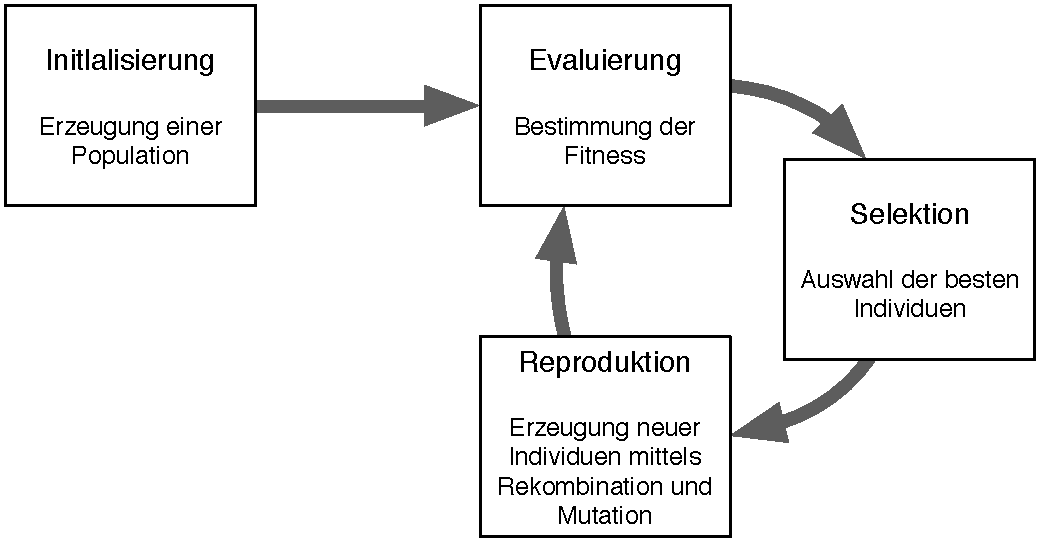
\includegraphics[width=0.8\textwidth]{evo_basic}
\caption{Ablauf evolutionärer Algorithmen}
\label{fig:evo_basic}
\end{figure}

Es handelt sich um heuristische Algorithmen, die das Finden einer optimalen Lösung nicht garantieren können \cite[S. 12]{gk2004}.

Grundsätzlich folgt das Vorgehen einem Kreislauf mit den Komponenten \emph{Evaluierung}, \emph{Selektion} und \emph{Reproduktion}. Nach Generierung einer anfänglichen Population (\emph{Initialisierung}) wird dieser Kreislauf so lange durchlaufen, bis ein vorher definiertes Abbruchkriterium eintritt. Ein Durchlauf wird als \emph{Generation} bezeichnet. Das Abbruchkriterium kann beispielsweise ein bestimmter Schwellwert für die Güte der Lösung oder eine feste Anzahl von Generationen sein. Der beschriebene Ablauf ist in \cref{fig:evo_basic} dargestellt.

Die einzelnen Komponenten eines evolutionären Algorithmus werden im Folgenden beschrieben. Die Definitionen folgen im Wesentlichen denen von \textcite{tw2008}.

\paragraph{Initialisierung}

Die Population \(P\) stellt eine Menge von Lösungskandidaten dar. Ein Lösungskandidat \(i\) wird als \emph{Individuum} bezeichnet und durch seinen \emph{Genotyp} repräsentiert. Der Genotyp ist die kodierte Repräsentation aller Variablen, die den Lösungskandidaten spezifizieren. Die Variablen werden \emph{Gene} genannt. Während der Initialisierung werden Lösungskandidaten erzeugt, die die Startpopulation des evolutionären Algorithmus bilden. Die Gene jedes Individuums werden üblicherweise zufällig gewählt.

\paragraph{Evaluierung}

Der Evaluierungsschritt dient zur Bestimmung der \emph{Fitness} der Individuen, die noch in der Population enthalten sind. Die Fitness stellt einen Wert dar, der die Güte der durch das Individuum repräsentierten Lösung bezüglich der Problemstellung beschreibt. Die Fitness eines Individuums \(i\) kann, je nach Optimierungsproblem, entweder absolut oder bezüglich der anderen Individuen der Population \(P\) bestimmt werden. Somit lässt sich die Funktion zur Bestimmung der Fitness auf die Form \(fitness(i, P)\) generalisieren.

\paragraph{Selektion}

Im Selektionsschritt werden die fittesten Individuen der Population \(P\) ausgewählt. Alle nicht ausgewählten Lösungskandidaten werden verworfen. Die Selektion kann als Funktion der Form \(select(P, fitness, s)\) dargestellt werden, wobei \(s\) eine festgelegte Anzahl von Individuen darstellt, die ausgewählt werden sollen.

\paragraph{Reproduktion}

Die Reproduktion dient dazu, aus den im Selektionsschritt ausgewählten Individuen neue Lösungskandidaten zu erzeugen. Dabei werden üblicherweise die Operationen \emph{Rekombination} und \emph{Mutation} verwendet. Bei der Rekombination wird, analog zur Biologie, aus zwei Elternindividuen ein neues Kindindividuum erzeugt. Sie lässt sich als Funktion der Form \(i_n = recombine(i_a, i_b)\) darstellen, wobei \(i_n\) das neue Individuum und \(i_a\) und \(i_b\) die Elternindividuen darstellen. Eine Mutation erzeugt ein neues Individuum durch die Modifikation eines anderen und ist daher durch die Funktion \(i_n = mutate(i_a)\) spezifiziert.

In der Literatur \cite{kw2007, tw2008, dj2006} finden sich für Selektion, Mutation und Rekombination Standardverfahren, die in Hinblick auf das zu lösende Optimierungsproblem ausgewählt werden können. Die konkret implementierten Verfahren werden in \cref{evo_implementation} beschrieben.

Nachdem evolutionäre Algorithmen grundlegend beschrieben wurden, wird im nächsten Abschnitt erläutert, wie die Priorisierung mittels dieser Algorithmenklasse implementiert werden kann.

\subsection{Anwendung zur Priorisierung}
\label{prio_evo}

Mit Hilfe von evolutionären Algorithmen kann der Prozess der Priorisierung aus \cref{prioritization} genauer beschrieben werden. \cref{fig:prioritization_evo} zeigt den Prozess mit den Komponenten evolutionärer Algorithmen.

\begin{figure}
\centering
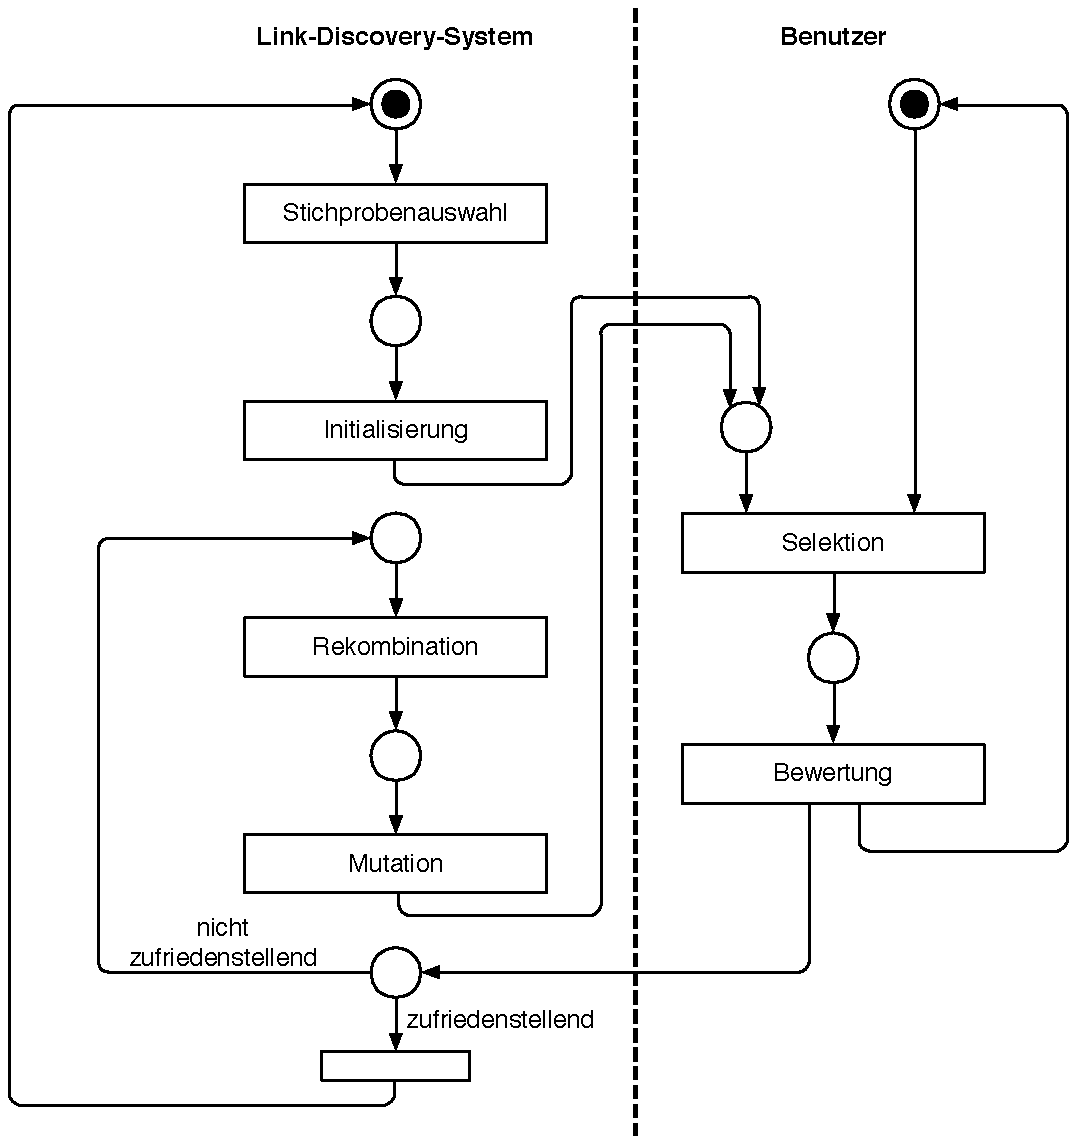
\includegraphics[width=0.8\textwidth]{prioritization_evo}
\caption{FMC--Petri--Netz der Priorisierung mittels evolutionärer Algorithmen}
\label{fig:prioritization_evo}
\end{figure}

Im Gegensatz zu \cref{fig:prioritization} ist zu erkennen, dass die Schritte zur Priorisierungserzeugung mit den Komponenten evolutionärer Algorithmen Initialisierung, Rekombination und Mutation ausgetauscht wurden. Die Selektion wird vom Benutzer vorgenommen, welcher anschließend bewertet, ob die ausgewählten Lösungskandidaten eine zufriedenstellende Priorisierung der Beziehungstypen darstellen.

Nach der Stichprobenauswahl wird für die Stichprobe eine Population von Lösungskandidaten erzeugt. Der Genotyp eines Individuums sollte pro Zusammenhangstyp ein Gewicht enthalten. Jedes Individuum stellt somit eine Gewichtung der Zusammenhangstypen dar.

Da der Algorithmus den Eingriff eines Benutzers erfordert, handelt es sich um einen \emph{interaktiven evolutionären Algorithmus} \cite{ht2001}. Die interaktive Komponente ist hierbei die Selektion, wodurch der Schritt der Evaluierung übersprungen werden kann. Wird die Selektion direkt vom Benutzer ausgeführt, erübrigt sich die Bestimmung eines Fitnesswertes.

Die Schritte der Rekombination und Mutation dienen zur Erzeugung neuer Lösungskandidaten auf Basis der vom Benutzer selektierten Priorisierungen. Sie sollten so gewählt werden, dass genügend unterschiedliche Priorisierungen erzeugt werden, aber dennoch eine Verbesserung über die Generationen erkennbar ist.

Zusammenfassend stellen evolutionäre Algorithmen eine geeignete Methode dar, um die Priorisierung durchzuführen, da die Schritte der Priorisierungserzeugung darauf abgebildet werden können. Die Stichprobenauswahl, die konkret implementierten Komponenten, die Durchführung der Selektion und die Ergebnisse werden in \cref{evo_implementation} detailliert erläutert.

\section{Zusammenfassung}

In diesem Kapitel wurde das Framework zur Link Discovery erläutert. Dies beinhaltet den modellierten Weltausschnitt und dessen Umsetzung auf eine Graph--Datenstruktur. Der Prozess der Erzeugung, Anreicherung und Priorisierung der Beziehungen dieses Modells wurde definiert und beschrieben. Zur Beziehungserzeugung wurde Kookkurrenz vorgestellt, die gängigen Maße genannt und die Berechnung erläutert. Ferner wurden mögliche Datenquellen für die Anreicherung diskutiert sowie der Einsatz evolutionärer Algorithmen zur Beziehungspriorisierung beschrieben. Nachdem in diesem Kapitel das Link--Discovery--Framework umfassend behandelt wurde, beschreibt das nächste Kapitel die konkrete Durchführung der Link Discovery.
